\documentclass{article}

\usepackage[utf8]{inputenc}

\usepackage[a4paper, total={6in, 9in}]{geometry}

\usepackage{hyperref}
\hypersetup{
    colorlinks=true,
    linkcolor=blue,
    filecolor=magenta,      
    urlcolor=blue,
}

\usepackage{graphicx}
\graphicspath{ {images/} }

\usepackage{listings}
\usepackage{xcolor}

\definecolor{codegreen}{rgb}{0,0.6,0}
\definecolor{codegray}{rgb}{0.5,0.5,0.5}
\definecolor{codepurple}{rgb}{0.58,0,0.82}
\definecolor{backcolour}{rgb}{0.95,0.95,0.92}

\lstdefinestyle{mystyle}{
    backgroundcolor=\color{backcolour},   
    commentstyle=\color{codegreen},
    keywordstyle=\color{magenta},
    numberstyle=\tiny\color{codegray},
    stringstyle=\color{codepurple},
    basicstyle=\ttfamily\footnotesize,
    breakatwhitespace=false,         
    breaklines=true,                 
    captionpos=b,                    
    keepspaces=true,                 
    numbers=left,                    
    numbersep=5pt,                  
    showspaces=false,                
    showstringspaces=false,
    showtabs=false,                  
    tabsize=2
}

\lstset{style=mystyle}

\title{POO - Tutoriat 2}
\author{Raluca Tudor şi Mihai-Dragoş Preda}
\date{18 Martie 2021}

\begin{document}

\maketitle

\section*{Recapitulare Tutoriat 1}
Să ne amintim lucrurile interesante prezentate în primul tutoriat:

\begin{itemize}
    \item Pointeri 
    
    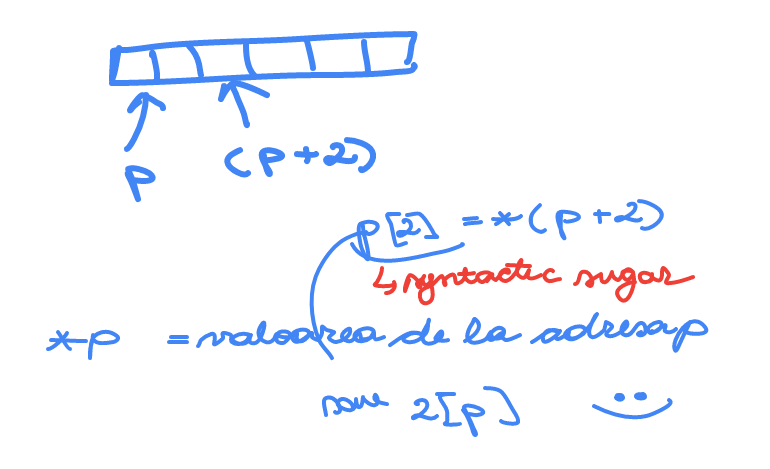
\includegraphics[scale=0.3]{desen1.png}
\end{itemize}

\begin{lstlisting}[language=C++]
#include <iostream>

using namespace std;

// ELEMENTE ALOCATE DINAMIC IN CLASA => COPY CONSTRUCTOR
class Vector {
private:
    int *v;
    int n;

public:
    Vector(int n) {
        this->n = n;
        v = new int[n];
    }

    Vector(const Vector& other) {
        cout << "Copy constructor\n";
        n = other.n;
        v = new int[n];
        for (int i = 0; i < n; i++)
            v[i] = other.v[i];
    }

    ~Vector() {
        delete[] v;
    };

    void setElement(int ind, int val) {
        v[ind] = val;
    }

    int getElement(int ind) {
        return v[ind];
    }

    int catePare() {
        int cnt = 0;
        for (int i = 0; i < n; i++)
            if (v[i] % 2 == 0)
                cnt++;
        return cnt;
    }

    void operator*=(int x) {
        for (int i = 0; i < n; i++)
            v[i] += x;
    }

    int& operator[](int x) {
        return v[x];
    }

    void operator=(const Vector &other) {
        cout << "operator=\n";
        delete[] v;
        n = other.n;
        v = new int[n];
        for (int i = 0; i < n; i++)
            v[i] = other.v[i];
    }
};

int main() 
{
    Vector* a = new Vector(5);
    a->setElement(3, 12);
    cout << a->getElement(3);

    delete a;
    return 0;
}
\end{lstlisting}

\begin{itemize}
    \item v += 10; \\
    este echivalent cu a scrie \\
    v.operator+=(10);
    \item v[0] = 1; \\
    este echivalent cu a scrie \\
    v.operator[](0) = 1;
    \item a-$>$setElement(3, 12); \\
    este echivalent cu a scrie \\
    (*a).setElement(3, 12);
\end{itemize}

\textbf{Foarte important!} Cazurile pe care se apelează \textbf{COPY CONSTRUCTOR}:

Presupunem că avem declarată instanţa v a clasei Vector.
\begin{enumerate}
    \item Vector v2(v);
    \item Vector v3 = v;
    \item afisare(v); // (Apel de funcţie)
\end{enumerate}

\section*{Tutoriat 2}



\subsection*{Extra întrebări}
\begin{itemize}
    \item \href{https://www.freelancer.com/community/articles/how-c-works-understanding-compilation}{How does compilation in C++ work?}
    \item \href{https://stackoverflow.com/questions/1452721/why-is-using-namespace-std-considered-bad-practice}{Why is “using namespace std;” considered bad practice?}
\end{itemize}

\end{document}
